\label{sec:dataaset}
\begin{figure*}[t!]
\centering
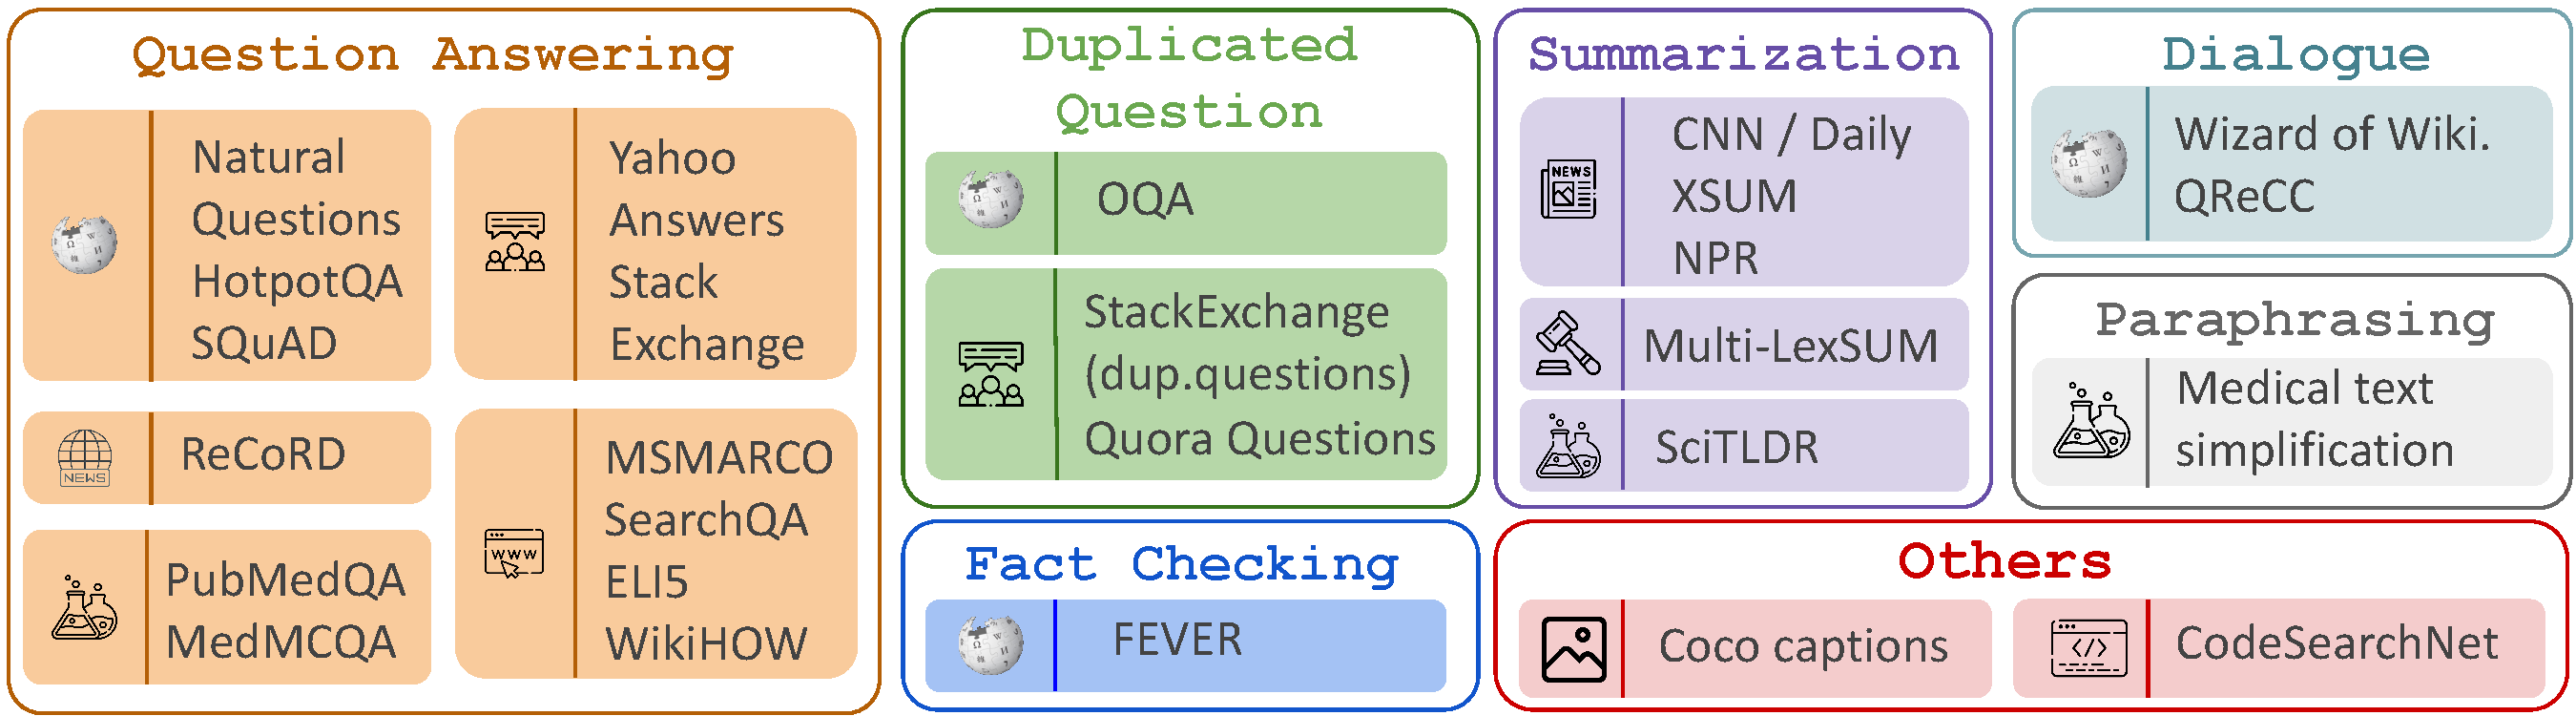
\includegraphics[width=0.95\textwidth]{imgs/dataset_figures_final.pdf}\caption{Examples of datasets included in \rib.} \label{fig:train_datasets}
\end{figure*}
To facilitate research in retrieval with natural language instructions, we build a unified large-scale retrieval dataset, \rib ({\bf B}ank of {\bf E}xplicit {\bf R}et{\bf R}ieval {\bf I}nstructions). 
{\rib consists of instructions and instances from diverse domains and tasks, by carefully curating retrieval datasets and casting diverse NLP datasets as retrieval tasks. }


\subsection{{Unified Task and Instructions Scheme }}
\paragraph{Task format.}
Each task $\mathcal{T}$ in \rib consists of a corpus $\mathcal{D}$, queries $\mathcal{Q} =\{\boldsymbol{q_1}, \ldots, \boldsymbol{q}_K\}$, and an instruction $\boldsymbol{t}$, where $K$ is the number of the queries included in the task.
An instance of each task includes a query $\boldsymbol{q}$, gold (relevant) documents $\boldsymbol{d}^{+}$, and negative (irrelevant) documents $\boldsymbol{d}^{-}$. 
For each task, an explicit intent $\boldsymbol{t}$, which can be paraphrased in multiple ways, is given. 
\paragraph{Instruction schema for retrieval.}
\label{sec:instruction_scheme}
Informative and diverse instructions are key for successful instruction tuning~\cite{sanh2022multitask}. 
{We introduce a novel scheme to define an informative instruction for retrieval tasks, which have not been studied in prior instruction-following literature. }
An instruction that sufficiently describes an arbitrary retrieval task should include: \emph{\hlc[pink]{intent}}, \emph{\hlc[cyan!30]{domain}} and \emph{\hlc[green!30]{unit}}.
{Specifically,} \emph{\hlc[pink]{intent}} describes how the retrieved text relates to the query, such as whether the text answers a question in the query or paraphrases it.
\emph{\hlc[cyan!30]{Domain}}  is the expected source or type of retrieved text, such as Wikipedia or PubMed articles. 
\emph{\hlc[green!30]{Unit}} defines the text block to retrieve, such as a sentence or a paragraph.
Table~\ref{tab:instructions} shows examples of instructions, and Appendix~\ref{sec:list_of_instructions} shows the full list.

\subsection{Dataset Collection}
\label{sec:dataset_collecitons}
\rib includes diverse datasets, including widely-used retrieval (e.g., MS MARCO;~\citealt{msmarco}), retrieval-centric datasets (NQ-open; \citealt{47761}) and non-retrieval datasets that can be repurposed as retrieval tasks. 
Figure~\ref{fig:train_datasets} shows the source datasets in \rib.  
{We manually annotate in multiple instructions per dataset}, and conduct multiple post-processing steps to provide a set of the query, gold, and negative documents. 
Table~\ref{tab:list_of_datasets} shows the full dataset list.
\paragraph{Selecting source datasets.}
We manually collect datasets from (1) KILT~\cite{petroni-etal-2021-kilt}, (2) the Sentence-Transformers Training Data for Text Embedding Models\footnote{\url{https://huggingface.co/datasets/sentence-transformers/embedding-training-data}}, and (3) manual searches in ACL anthologies and huggingface datasets\footnote{\url{https://huggingface.co/docs/datasets/index}} to cover a diverse set of tasks and domains. 
{
We observe that except for a few domains (e.g., Wikipedia) many domains do not have retrieval datasets while there are a few datasets for other NLP tasks that can be cast as retrieval (e.g., sentence paraphrase). 
Re-purposing those non-retrieval tasks as retrieval tasks enables to diversity of the domains as well as the instructions in \rib.  
}

From an initial list of more than {60} datasets, we assess whether it is suitable for repurposing as a retrieval task. Specifically, we sample 20 instances from the candidate dataset and check if the queries are self-contained.\footnote{For examples, finding a corresponding review text for the review title ``{\it I love this!}'' is under-specified.}
If the majority of queries fail this test, we exclude the corresponding dataset.
%
%
Consequently, we use 37 datasets, including more than {5 million} instances in total. 
For datasets that are orders of magnitude larger than other datasets (e.g., PAQ; \citealt{lewis-etal-2021-paq}), we randomly sample up to 300k instances, except for MS MARCO.\footnote{Prior work has shown that MS MARCO can be beneficial to many downstream retrieval tasks~\cite{izacard2022unsupervised}.}
As a result, \rib covers diverse domains (e.g., Wikipedia, scientific papers) and tasks (e.g., fact verification, dialogue response retrieval, QA). See Appendix~\ref{sec:dataset_analysis} for more details.

\begin{figure*}[t!]
\centering
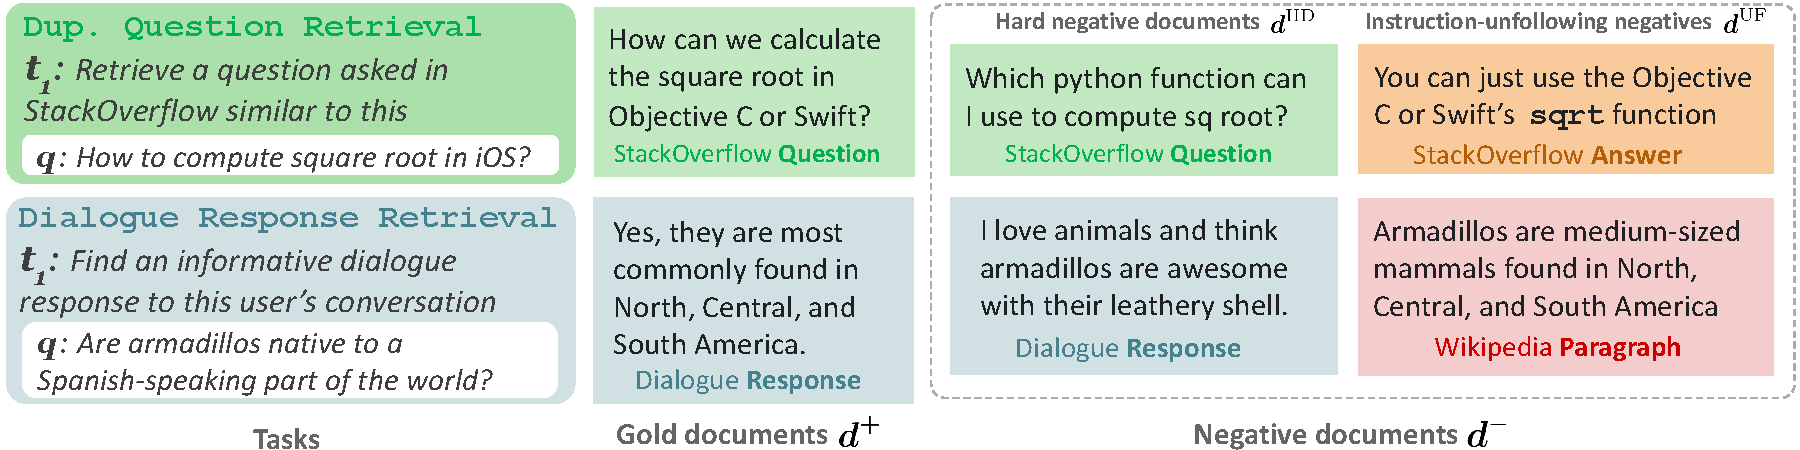
\includegraphics[width=\textwidth]{imgs/exmample_figures_final.pdf}\caption{Examples of documents that are considered gold documents $\boldsymbol{d}^+$, and two types of negative documents $\boldsymbol{d}^-$: hard negatives $\boldsymbol{d}^{\rm HD}$ and instruction-unfollowing negatives $\boldsymbol{d}^{\rm UF}$ for two different query and instruction pairs. 
} \label{tab:dataset_schema}
\end{figure*}
\paragraph{{Unification and instruction annotations.}}
{
For retrieval datasets such as MS MARCO, we use the annotated gold documents as positive documents $\boldsymbol{d}^{+}$ to a given query $\boldsymbol{q}$. 
Regarding non-retrieval tasks, we use the original input sequence as a query $\boldsymbol{q}$ and the original output or given context as $\boldsymbol{d}^{+}$. 
{For instance, given a summarization dataset we use a source text and a summary as a query and a gold document, respectively. }}

For each dataset, the authors of this paper manually wrote {instructions ({8 maximum and 3.5 average number of instructions per task).}
For datasets without preprocessed retrieval targets,\footnote{For example, KILT datasets such as FEVER or NQ use the unified Wikipedia corpus. } we gather all positive and negative documents provided by the original dataset to build a single task-specific retrieval corpus $\mathcal{D}$.
{
More details are described in Appendix Section~\ref{sec:unification}. 
}

\paragraph{{Negative documents selection.}}
Negative samples are crucial for training retrieval systems~\cite{zhan-2021-optimizing}. 
{
In addition to the randomly sampled negative samples (random negative documents), we introduce two types of challenging negative samples: denoised hard negative documents $\boldsymbol{d}^{\rm HD}$ and instruction-unfollowing negative documents $\boldsymbol{d}^{\rm UF}$.}
Figure~\ref{tab:dataset_schema} shows examples of gold documents, hard negatives, and instruction-unfollowing documents. 

We mine hard negative documents $\boldsymbol{d}^{\rm HD}$ using an off-the-shelf retriever and then filter out false negative documents using an off-the-shelf reranker, following \citet{qu-etal-2021-rocketqa}. 
{In particular, we retrieve top documents from the target corpus using Contriever~\cite{izacard2022unsupervised} and then add new documents whose normalized scores predicted by a cross-encoder model, \texttt{ms-marco-MiniLM-L-12-v2}\footnote{\url{https://huggingface.co/cross-encoder/ms-marco-MiniLM-L-12-v2}} are below 0.1 as hard negative documents. }


We further introduce a new negative sampling strategy, instruction-\emph{unfollowing} negative samples $\boldsymbol{d}^{\rm UF}$, to make systems learn to \emph{follow} instructions and retrieve documents that align with the specified intents.
As shown in Figure~\ref{tab:dataset_schema}, given an instruction ``find an informative dialogue response'', a system should not retrieve a Wikipedia paragraph about armadillos. 
To obtain those instruction-unfollowing negative documents, we retrieve documents from a different task's target corpus using the same off-the-shelf Contriever and consider all those documents to be negatives since they do not satisfy the instruction.
More details about instruction-unfollowing negatives are in Appendix Section~\ref{sec:details_of_negative}. 